\section{High Order Logic and Model Checking}

Verfiying complex computer systems requires propostional temporal logics. 
Time in these forms of logic can be reprented linear or branching. Time means the order of events e.g. \glqq The message has been send after receiving. \grqq
In model checkes these forms of high order logic are applied.
In pricatical applications these times have no imcat in the real execution time of events (e.g. $3 \mu sec$. Moreover real-time systems time-contraight of asyncronus systems require{\itshape compuational tree logic} (CTL).\cite{BK}
\begin{figure}[h]
		\centering
		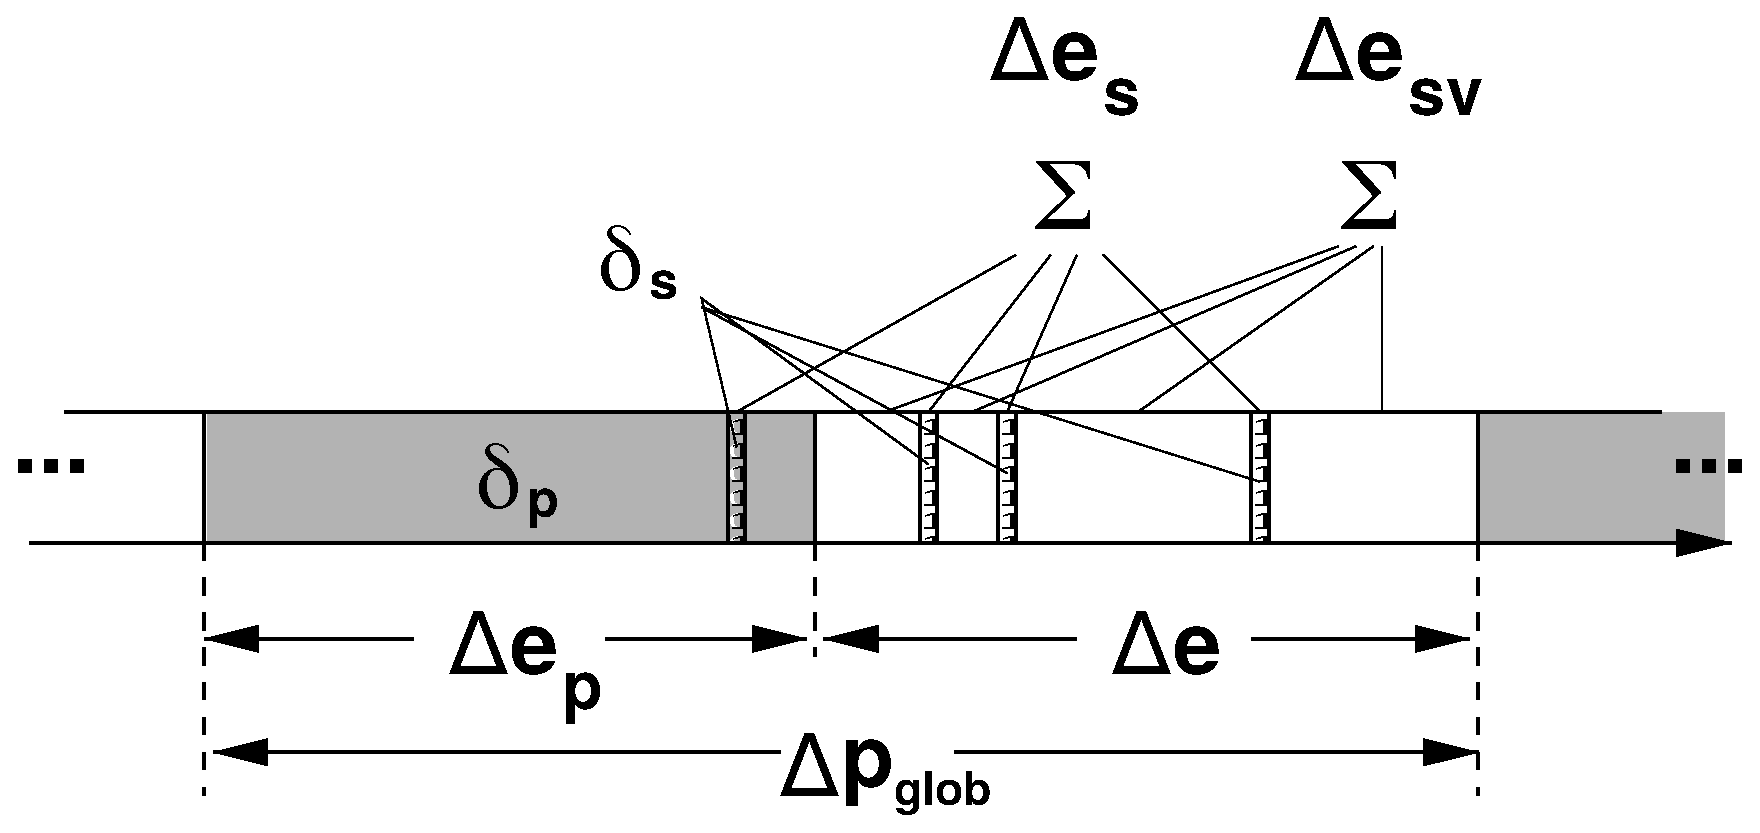
\includegraphics[width=0.7\textwidth]{timeslot_and_disruptive_process.eps}
		\caption{Timeslot partitioning of  $\Delta e_s, \Delta e_p$, $\Delta e_{sv}$ and $\Delta_e$ of the disruptive process $\delta_s$ and $\delta_p$, Source: \cite{BK}}
		\label{fig:timeslots}
\end{figure}

Example question from the textbook, which can be solved applying LTL  \cite[Chapter 5]{BK}.

Solve the following questions concerning the leader election protocol:

\begin{enumerate}
	\item Model Peterson’s leader election protocol in Promela (avoid invalid end states).
	\item  Verify the following properties:
	\item There is always at most one leader.
	\item Eventually always a leader will be elected.
	\item The elected leader will be the process with the highest number.
	\item The maximum total amount of messages sent in order to elect a leader is at most $2N \lfloor log 2 N \rfloor  + N$.
\end{enumerate}


\begin{table}[h]
		\begin{left}
			\begin{tabular}{l|l}
	 		logic  &  linear time  &  branching-time  & real-time requirement  \\ 
	 		       &  (path-based) &  (state based)   & (continous-time-doamin) \\  \hline 
		           &   \checkmark  &                  &                         \\  
		     	   &               &  \checkmark      &     \checkmark          \\  
		     	   &               &  \checkmark       &    \checkmark          \\   
	        \end{tabular}
		\end{left}
		\label{tab:CoqAndPreciateLogic}
		\caption{classification of temporal logics in \cite{BK} } 
	\end{table}
complexity of model checking problems
p. 314 book

